% Options for packages loaded elsewhere
\PassOptionsToPackage{unicode}{hyperref}
\PassOptionsToPackage{hyphens}{url}
%
\documentclass[
  11pt,
  a4paperpaper,
]{article}
\usepackage{lmodern}
\usepackage{amsmath}
\usepackage{ifxetex,ifluatex}
\ifnum 0\ifxetex 1\fi\ifluatex 1\fi=0 % if pdftex
  \usepackage[T1]{fontenc}
  \usepackage[utf8]{inputenc}
  \usepackage{textcomp} % provide euro and other symbols
  \usepackage{amssymb}
\else % if luatex or xetex
  \usepackage{unicode-math}
  \defaultfontfeatures{Scale=MatchLowercase}
  \defaultfontfeatures[\rmfamily]{Ligatures=TeX,Scale=1}
  \setmainfont[]{Carlito}
\fi
% Use upquote if available, for straight quotes in verbatim environments
\IfFileExists{upquote.sty}{\usepackage{upquote}}{}
\IfFileExists{microtype.sty}{% use microtype if available
  \usepackage[]{microtype}
  \UseMicrotypeSet[protrusion]{basicmath} % disable protrusion for tt fonts
}{}
\makeatletter
\@ifundefined{KOMAClassName}{% if non-KOMA class
  \IfFileExists{parskip.sty}{%
    \usepackage{parskip}
  }{% else
    \setlength{\parindent}{0pt}
    \setlength{\parskip}{6pt plus 2pt minus 1pt}}
}{% if KOMA class
  \KOMAoptions{parskip=half}}
\makeatother
\usepackage{xcolor}
\IfFileExists{xurl.sty}{\usepackage{xurl}}{} % add URL line breaks if available
\IfFileExists{bookmark.sty}{\usepackage{bookmark}}{\usepackage{hyperref}}
\hypersetup{
  hidelinks,
  pdfcreator={LaTeX via pandoc}}
\urlstyle{same} % disable monospaced font for URLs
\usepackage[margin = 3cm]{geometry}
\usepackage{graphicx}
\makeatletter
\def\maxwidth{\ifdim\Gin@nat@width>\linewidth\linewidth\else\Gin@nat@width\fi}
\def\maxheight{\ifdim\Gin@nat@height>\textheight\textheight\else\Gin@nat@height\fi}
\makeatother
% Scale images if necessary, so that they will not overflow the page
% margins by default, and it is still possible to overwrite the defaults
% using explicit options in \includegraphics[width, height, ...]{}
\setkeys{Gin}{width=\maxwidth,height=\maxheight,keepaspectratio}
% Set default figure placement to htbp
\makeatletter
\def\fps@figure{htbp}
\makeatother
\setlength{\emergencystretch}{3em} % prevent overfull lines
\providecommand{\tightlist}{%
  \setlength{\itemsep}{0pt}\setlength{\parskip}{0pt}}
\setcounter{secnumdepth}{5}
\usepackage{placeins}
\usepackage{booktabs}
\usepackage{carlito}
\usepackage{array}
\usepackage{chngcntr}
\usepackage{color}
\usepackage{titlesec}
\usepackage{titling}
\usepackage{caption}
\usepackage[bottom]{footmisc}
\usepackage[justification = centering]{caption}
\usepackage{lscape}
\usepackage{pdflscape}
\usepackage{longtable}
\usepackage{threeparttable}
\usepackage{nopageno}
\usepackage{footnote}

\counterwithin{figure}{section}
\counterwithin{table}{section}
\definecolor{ESSPink}{rgb}{0.91,0.2,0.32}


\titleformat
	{\section}
	{\bf \LARGE \sc \color{ESSPink}}
	{\rlap{\thesection}\hspace{1cm}}
        {0pt}
        {}
	[{\titlerule[2pt]}]

\titleformat
	{\subsection}
	{\bf \large \sc}
	{\rlap{\thesubsection}\hspace{1cm}}
	{0pt}
        {}

\newcommand*{\secref}[1]{Section~\ref{#1}}

\captionsetup[figure]{labelfont= {color = ESSPink, bf}, labelsep = space}
\captionsetup[table]{labelfont= {color = ESSPink, bf}, labelsep = space}

\let\stdsection\section
\renewcommand{\section}{\FloatBarrier\clearpage\FloatBarrier\stdsection}

\newcommand{\blandscape}{\begin{landscape}}
\newcommand{\elandscape}{\end{landscape}}
\usepackage{titling}
\setlength{\droptitle}{5em}
\usepackage{booktabs}
\usepackage{longtable}
\usepackage{array}
\usepackage{multirow}
\usepackage{wrapfig}
\usepackage{float}
\usepackage{colortbl}
\usepackage{pdflscape}
\usepackage{tabu}
\usepackage{threeparttable}
\usepackage{threeparttablex}
\usepackage[normalem]{ulem}
\usepackage{makecell}
\usepackage{xcolor}
\ifluatex
  \usepackage{selnolig}  % disable illegal ligatures
\fi
\newlength{\cslhangindent}
\setlength{\cslhangindent}{1.5em}
\newlength{\csllabelwidth}
\setlength{\csllabelwidth}{3em}
\newenvironment{CSLReferences}[2] % #1 hanging-ident, #2 entry spacing
 {% don't indent paragraphs
  \setlength{\parindent}{0pt}
  % turn on hanging indent if param 1 is 1
  \ifodd #1 \everypar{\setlength{\hangindent}{\cslhangindent}}\ignorespaces\fi
  % set entry spacing
  \ifnum #2 > 0
  \setlength{\parskip}{#2\baselineskip}
  \fi
 }%
 {}
\usepackage{calc}
\newcommand{\CSLBlock}[1]{#1\hfill\break}
\newcommand{\CSLLeftMargin}[1]{\parbox[t]{\csllabelwidth}{#1}}
\newcommand{\CSLRightInline}[1]{\parbox[t]{\linewidth - \csllabelwidth}{#1}\break}
\newcommand{\CSLIndent}[1]{\hspace{\cslhangindent}#1}

\author{}
\date{\vspace{-2.5em}}

\begin{document}

\newpage
\FloatBarrier
\pagenumbering{gobble}

\begin{titlepage}
    \raggedleft
    
\includegraphics[width = 6cm]{ESSlogo.png}
    \vfill
    \raggedright
    {\bf \fontsize{40pt}{50pt}\selectfont Interim Dataset Analysis, Round 11}\\[1 cm]
    {\sc \fontsize{20pt}{30pt}\selectfont Report of Standardised Analysis for Detection of Interviewer-Controlled Issues}\\[1 cm]
    \vfill
    \begin{center}\large
    ESS ERIC Core Scientific Team\footnote[1]{Authors: Roberto Briceno-Rosas (GESIS Leibniz Institute for the Social Science in Mannheim, Germany), May Dousak (University of Ljubljana, Slovenia), Paulette Flore and Joost Kappelhof (SCP - The Netherlands Institute for Social Science Research, The Netherlands) / For internal distribution only.}
    \end{center}
    \begin{center}
    {\large \today}
    \end{center}
\end{titlepage}

\pagenumbering{arabic}

\setcounter{tocdepth}{2}
\tableofcontents
\listoffigures

\begin{verbatim}
## Error in `dplyr::select()`:
## ! Can't subset columns that don't exist.
## x Column `intnum` doesn't exist.
\end{verbatim}

\begin{verbatim}
## Error in is.data.frame(y): object 'Inwer_ID' not found
\end{verbatim}

\hypertarget{readers-guide}{%
\section*{Reader's Guide}\label{readers-guide}}
\addcontentsline{toc}{section}{Reader's Guide}

This report presents the results of the analysis of the interim dataset
for NA. It aims to help national teams detecting undesirable interviewer
behaviour in a timely manner. The report has been standardised for
implementation in all participating countries as remote analysis of the
interim dataset without the intervention of the international ESS team
and without having to move securely stored data from the national level.
The report focuses on indicators expected to signal issues with
undesirable interviewer behaviour but it can also help detect other
issues regarding data collection which are not related to interviewer
behaviour. The reader's guide explains how to best utilize the report
and take the appropriate steps for data colleciton. It is highly
encourage to keep close communication with the CST via the Country
Contact for discussion of results and consultation regarding any
important decision. Please share the report with your Country Contact.
This report should also be stored and deposited for documentation
purposes along the data and other respective documents to the ESS
Archive after fieldwork has been completed.

\hypertarget{theorical-background}{%
\subsection{Theorical Background}\label{theorical-background}}

Interviewers can have a systematic and substantial impact on the
resulting data. Sometimes, their impact is beyond their control, for
example, respondents might answer questions somewhat differently when
interviewed by a male interviewer compared to when interviewed by a
female interviewers. Other times, their impact is well within their
control and it is a direct consequence of their behaviour. When
analyzing the interim datasets, we want to focus on
interviewer-controlled issues, which can be corrected for during the
fieldwork if necessary.

\emph{Types of interviewer-controlled issues}

Interviewer-controlled issues varied depending on the level of control
an interviewer has over it and the causes of the issue. One
classification used in the ESS to gain a better understanding of the
different ways undersirable interviwer behaviour can occurred is
provided by Stoop et al (\protect\hyperlink{ref-stoop2018}{2018}):

\begin{itemize}
\tightlist
\item
  Undesirable interviewer behaviour driven by context: Some examples are
  speeding through the interview when the respondent seems close to
  breaking off the interview, chatting with respondents who are unsure
  about their answers, paraphrasing a question when the respondent
  misunderstands, etc. In these cases, the interviewer depart from the
  expected behaviour due to an external element, for which the
  interviewer has little control of. They can be considered unavoidable
  to some extend, although in some situations the reaction of the
  interviewer could be improved to meet the desirable behaviour. More
  importantly, these issues should not be systematically related to the
  interviewer, but case-specific instead.
\item
  Undesirable interviewer behaviour that could be avoided: Some examples
  of these type of behavior are speeding through the interview, skipping
  introductions to questions, forgetting to hand over showcards, not
  properly reading answer categories, etc.
\item
  Unintentional errors: like erroneously interviewing the wrong person,
  recording the wrong day for the interview, keying the wrong answer
  category, etc.
\item
  Deliberate falsification: curbstoning (creating the answers for an
  entire or partial interviews), partially duplicating interviews
  (copying answers), selecting available household members as
  respondents instead of a random member of the household because they
  are more cooperative or more often at home when the interviewer
  contacts the sample unit, incorrectly recording answers to filter
  questions to reduce the duration of the survey, etc. In the cases, the
  behaviour is intentional and constitute a depature from the standards
  of survey interviewing set by the ESS.
\end{itemize}

Understanding the type of interviewer-controlled issues is important for
deciding the course of action. For example, an interviewer who
mistakenly missed parts of the questionnaire might require better
training or briefing on the ESS questionnaire, while an interviewer who
skipped parts of the questionnaire to save time might need to be
excluded from the fieldwork activities. Data analysis can provide clues
about the type of issues and help focus the monitoring efforts. However,
further investigation is most likely necessary to assert the type of
behaviour that caused the issues.

\emph{Prevention and detection}

One of the key steps for successful promotion of desirable interviewer
behaviour is detecting issues in the field as early as possible.
Detection leads to prevention of further issues and therefore to
mitigation of the impact of undesirable interviewer behaviour. Even if
issues can not be corrected, understanding the causes that lead to issue
allows to make better informed decision and document problems for data
users. The more time it has passed between the detection of a data
issues and the fieldwork, the harder it is to understand the issue.

\emph{Strategies for dectecting interviewer-controlled issues}

Data analysis of interim datasets is one out of multiple strategies that
can be used to detect interviewer-controlled issues during data
collection. Other strategies include observation of interviewer
behaviour in the field, interviewer debriefing, or back-checks or
recontact sample units, analysis of fieldwork paradata (e.g.~contact
forms data), or activity tracking mechanism. Therefore, the interim
dataset from the main questionnaire is provides ``one piece of the
puzzle'' when attempting to reconstruct fieldwork activities in the
process of data collection and understand.

\emph{Standardised v country-specific analysis}

Standardised data analysis provides a basis for detection of issues
related to interviewer issues. It also allows international surveys like
the ESS to establish a minimum quality benchmark that is applied in all
participating countries and serves to improve comparability across
countries. However, standardised analysis for all participating
countries cannot account for country-specific characteristics that are
particular to national or regional context, specific survey design
characteristics, cultural background, technical particularities of the
tool used for the national teams for data collection o country-specific
fieldwork decision. It is highly encourage to interpret, adapt and
conduct further analysis that would address particular concerns expected
in each country.

\hypertarget{methods}{%
\subsection{Methods}\label{methods}}

\emph{Areas of Analysis}

Three areas of analysis have been defined in this report. The first
section presents the results on the analysis of the timestamps from the
interview. The second section focuses on item non-response. The third
section investigates response patterns of respondents and how these
related to allocations within interviewers.

\emph{Quality Benchmarks (flags)}

The quality benchmarks, also known as flags, function as default
threshold for each indicators presented in the report. Their purpose is
focusing the attention to possible issues rated to interviewer
behaviour. These benchmarks are arbitrary and they has been defined
based on experience of fieldwork activities across participant
countries. The thresholds are by no means fixed and they can be revised
to meet country-specific needs and fieldwork characteristics.

For the interim dataset, quality benchmarks have been defined with a low
sensitivity, meaning that is expected that higher number of cases will
be flag without an actual problem having ocurred (false positives). The
flag aim is to raise attention about possible issues for further
investigation, instead of reporting the existence of an issue \emph{per
se}.

\hypertarget{evaluation-of-results}{%
\subsection{Evaluation of Results}\label{evaluation-of-results}}

\_Figures, Tables and Detailed Tables in Annex Folder\_\_

In the report, results are presented in figures and table to provide a
quick overview of the issues. Promatic cases or interviewer are usually
highlighted. However, it is not always possible to provide a adaquate
overview of all issues for all countries. Therefore, indicators are
saved into the Annex folder together with the report for further
invatigation.

\emph{Adjustment of Quality Benchmarks}

Adjustment of the quality benchmarks might be necessary to better tune
to sensibility to country-specific context or to conduct a more focused
investigation of issues. There are two ways to adjust the quality
benchmarks used as default for this report: (1) recoding of the

\hypertarget{further-investigation}{%
\subsection{Further Investigation}\label{further-investigation}}

All flags provided by this report are granted further consideration and
investigation with the goal of gaining understanding about the causes of
the issues. The steps and efforts will depend on the type of flag and
the related level of concern.

\emph{Contextualization}

National teams and survey agencies have access to important information
about fieldwork activities, which this report does not account for. For
example, prior issues with specific interviewers or details about
specific geographical area of sample units can substantially influence
the levels of concern raised by flags. Therefore, the first step for the
national teams should be to contextualize the reported flags with
information available about fieldwork, including the characteristics of
the interviewers, the sample units, the details of the CAPI-system,
recent fieldwork activities, etc. The information required for
contextualization will depend on the respective quality benchmarks and
possible explanation for their occurrence. For example, the expected
travel distance between two sample units can provide crucial information
when asserting the feasibility of very short interval of time between
two interviews from the same interviewer.

\emph{Debriefing of Interviewers}

An important step in clarifying the issues is to query interviewer about
possible explanation of the issues observed. Interviewers are one of the
most important source of information for explaining issues observed in
the data as they were present in the production of the data. They can
help reconstruct the fieldwork activities that lead to the issues
observed. They should also be seen as partners in solving the issue as
their future behaviour might help avoid problem. We recommend that this
interaction takes place in a constructive and respectful manner as it.
We recommend to document the debriefing results in a short minute that
could help later in the assessment, especially if back-checks are
conducted.

\emph{Back-checks}

Please follow the ESS guidance on conducting the back-checks. Please
note that when conducting back-checks with the aim of clarifying
specific interviewer-related issues, you might need to ask the sample
units about specific information that clarifies the issues. For example,
if there are concern about parts of the questionnaire not having been
asked, you might need to ask the respondent whether they recall being
asked about those specific topics and present one or more of the
questions to help them recall.

\hypertarget{implications}{%
\subsection{Implications}\label{implications}}

\emph{Course of Action, Discussion and Documentation}

Once an understanding of the issues has been establish, it is time to
decide and discuss the course of action. The course of action should
always be decided on the case-by-case approach, considering all
available information and with the discussion with the respective
stakeholders. Some example of course of action might involve management
of the interviewers, like for example re-briefing, re-training,
supervised interviewing exercises, or removal of interviewers from field
activities. Management of the interviewers are under the responsibility
of the national team and survey agency, however, consultation with the
CST is encouraged. Other solutions might require a adjustment of the
survey design or manipulation of the data, like recontacting sample
units, correction of erroneous data, removal of data (partial or
complete), redrawing the sample. Please note that any course of action
that involved the modification of the fieldwork plans, contact strategy,
manipulation of data, or sampling design are not to be taken lightly and
need to be consulted with the Core Scientific Team before any action is
taken.

In some cases, the course of action might just be the documentation of
the issues, their probable cause, and the step taken to clarify the
issues. This allows the ESS to provide explanation to data users about
possible issues they might spot when making use of the data. It is
recommended to document any course of action taken as a results of
quality control and flags raised by this report.

\hypertarget{results-for-na}{%
\section{Results for NA}\label{results-for-na}}

The data provided to the tool contained a total of 2478 cases and a
total of 2477 contained a valid interviewer number. It should also be
noted that the analysis focused only on cases that have a valid
interviewer number as it is assumed that all interviews have been
conducted by an interviewer. Therefore, any case missing the interviewer
number are not included in the analysis.

\begin{table}[!h]

\caption{\label{tab:nperm}\label{tab:table_nperm} Descriptive summary of interviews per interviwer}
\centering
\begin{tabular}[t]{r|r|r|r|r|r|r|r}
\hline
min & max & mean & sd & Q1 & Q2 & Q3 & n\\
\hline
2 & 25 & 11.3105 & 4.722 & 8 & 10 & 14 & 219\\
\hline
\end{tabular}
\end{table}

\begin{figure}[H]
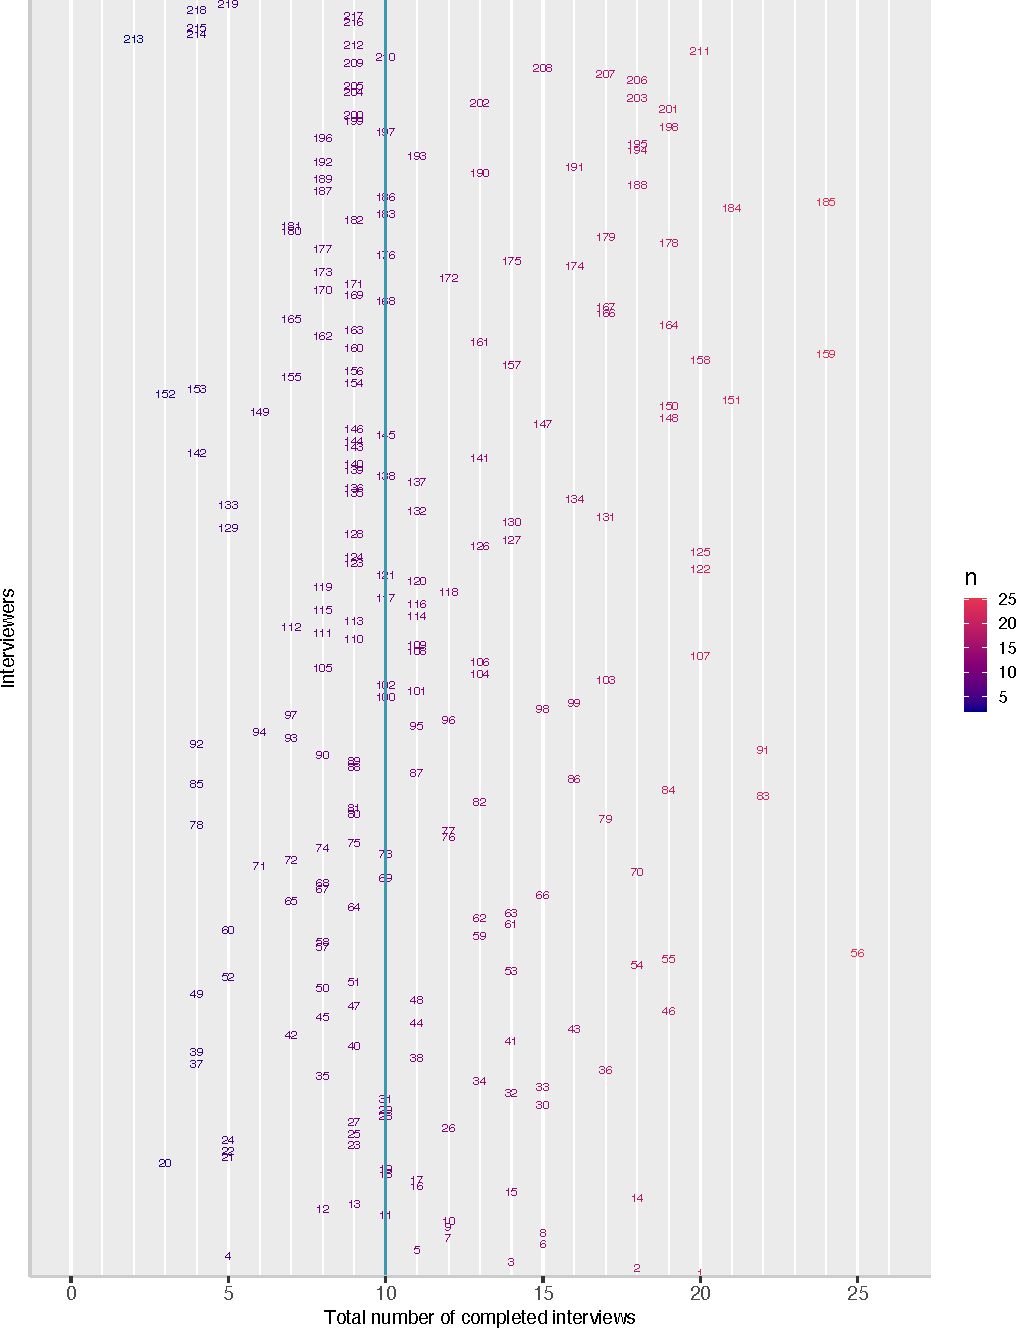
\includegraphics{Analysis_InterimD_R11_R10example-sav_files/figure-latex/nperm_plot-1} \caption[Distribution of interviews per interviewer]{\label{fig:nperm_plot} Distribution of interview per interviewer \hspace{\textwidth} Note: The vertical blue line represents the median number of completed interviews}\label{fig:nperm_plot}
\end{figure}

\hypertarget{sec:timestamps}{%
\section{Interview timestamps}\label{sec:timestamps}}

\begin{verbatim}
## Error in .local(x, ...): unused argument (origin = "1582-10-14")
\end{verbatim}

\begin{verbatim}
## Error in .local(x, ...): unused argument (origin = "1582-10-14")
\end{verbatim}

\begin{verbatim}
## Error in .local(x, ...): unused argument (origin = "1582-10-14")
\end{verbatim}

\begin{verbatim}
## Error in .local(x, ...): unused argument (origin = "1582-10-14")
\end{verbatim}

\begin{verbatim}
## Error in .local(x, ...): unused argument (origin = "1582-10-14")
\end{verbatim}

\begin{verbatim}
## Error in .local(x, ...): unused argument (origin = "1582-10-14")
\end{verbatim}

\begin{verbatim}
## Error in .local(x, ...): unused argument (origin = "1582-10-14")
\end{verbatim}

\begin{verbatim}
## Error in .local(x, ...): unused argument (origin = "1582-10-14")
\end{verbatim}

\begin{verbatim}
## Error in .local(x, ...): unused argument (origin = "1582-10-14")
\end{verbatim}

\begin{verbatim}
## Error in .local(x, ...): unused argument (origin = "1582-10-14")
\end{verbatim}

\begin{verbatim}
## Error in .local(x, ...): unused argument (origin = "1582-10-14")
\end{verbatim}

In this section, indicators for detection of issues in interviewing
process are drawn from the analysis of timestamps recorded for each
interview (start and end of the interview, including timestamps for each
module, and date and time of interview). Timestamps provide critical
information about the conduction of the interview in the field and can
help detect issues in the interviewing process.

First, we look at the interview duration and interview speed on both the
interview level and module level. Second, we analyze the time of the
interview relative to the time of other interviews from the same
interviewer. Please note that any issues highlighted require further
investigation by the national teams.

Countries that follow the recommendation of including more detailed
timestamps (e.g.~timestamps per item) into their CAPI systems are able
to conduct further analysis on those indicators. The ESS DIB team can
provide further assistance if needed.

\hypertarget{sec:duration_speed}{%
\subsection{Interview duration and interview
speed}\label{sec:duration_speed}}

Interview duration refers to the length of the interview excluding
optional country-specific questions, the interviewer questions, and
general administration of the contact procedures. Interview speed refers
to the average speed (in terms of question per minute) in which the
interview progresses. The average interview speed is calculated as the
number of applicable questions for a specific respondent divided by the
duration of the interview. It can be calculated at the interview level
or another level, such as the module level (see \secref{sec:speed}).

Both duration and speed should be considered when assessing data
quality. For example, extreme outliers in interview duration and/or
interview speed can indicate a deviation from interviewing protocols
(e.g.~error in the recording of timestamps) or even falsification of
interviews.

\hypertarget{sec:duration}{%
\subsubsection{Unlikely interview duration}\label{sec:duration}}

Very short or very long interviews can be attributed to interviewer
behaviour, but also to technical problems (e.g., software problems),
atypical interviews, or respondent behaviour (e.g., partial interviews)
(see \protect\hyperlink{ref-vandenplas2019}{Vandenplas, Beullens, \&
Loosveldt, 2019, p. 252}). Detecting outliers can help identify
systematic issues related to interviewers as a whole. Therefore, it is
important to consider all interviews conducted by interviewers that have
produced interviews with an unlikely duration. As mentioned before, very
short of very long interview durations (i.e., outliers) could indicate a
potential problem and in this analysis we define short interviews as
interviews having lasted less than 30 minutes and long interviews as
interviews having lasted 180 minutes or more.

\begin{verbatim}
## Error in `$<-.data.frame`(`*tmp*`, int_period, value = new("Interval", : replacement has 0 rows, data has 2477
\end{verbatim}

\begin{verbatim}
## Error in `$<-.data.frame`(`*tmp*`, duration, value = numeric(0)): replacement has 0 rows, data has 2477
\end{verbatim}

\begin{verbatim}
## Error in `dplyr::filter()`:
## ! Problem while computing `..1 = duration < 30`.
## Caused by error in `duration < 30`:
## ! comparison (3) is possible only for atomic and list types
\end{verbatim}

\begin{verbatim}
## Error in eval(expr, envir, enclos): object 'duration_30' not found
\end{verbatim}

\begin{verbatim}
## Error in `dplyr::filter()`:
## ! Problem while computing `..1 = duration > 180`.
## Caused by error in `duration > 180`:
## ! comparison (6) is possible only for atomic and list types
\end{verbatim}

\begin{verbatim}
## Error in eval(expr, envir, enclos): object 'duration_180' not found
\end{verbatim}

\begin{verbatim}
## Error in eval(expr, envir, enclos): object 'duration_30_vec' not found
\end{verbatim}

\begin{verbatim}
## Error in eval(expr, envir, enclos): object 'duration_improb' not found
\end{verbatim}

\begin{verbatim}
## Error in list2(...): object 'duration_30' not found
\end{verbatim}

\begin{verbatim}
## Error in df_duration_improb$intnum %in% duration_30_vec: object 'df_duration_improb' not found
\end{verbatim}

\begin{verbatim}
## Error in select(df_duration_improb, idno, intnum, unlikely_duration): object 'df_duration_improb' not found
\end{verbatim}

\begin{verbatim}
## Error in dplyr::count(., unlikely_duration, intnum): object 'df_duration_improb' not found
\end{verbatim}

\begin{verbatim}
## Error in `filter()`:
## ! Problem while computing `..1 = duration < 240`.
## i The error occurred in group 1: intnum = 1.
## Caused by error in `duration < 240`:
## ! comparison (3) is possible only for atomic and list types
\end{verbatim}

\begin{verbatim}
## Error in factor(df_duration$intnum, levels = unique(df_duration$intnum[order(df_duration$duration_mean)])): object 'df_duration' not found
\end{verbatim}

\begin{verbatim}
## Error in df_duration$intnum %in% duration_30_vec: object 'df_duration' not found
\end{verbatim}

\begin{verbatim}
## Error in psych::describe(df_duration$duration, quant = c(0.25, 0.75)): object 'df_duration' not found
\end{verbatim}

An overview of the distribution of interview duration by interviewer can
be seen in Figure \ref{fig:plot_duration}. Table
\ref{tab:table_duration} shows the frequencies of an interview with
unlikely duration per interviewer. For more details, see table in the
annex folder with the interview duration per case and interviewer
(``Interview duration.csv'').

\begin{verbatim}
## Error in `[.data.frame`(Main, , c("idno", "intnum", "int_period", "duration")): undefined columns selected
\end{verbatim}

\begin{verbatim}
## Error in ggplot(df_duration, aes(duration, as.factor(intnum))): object 'df_duration' not found
\end{verbatim}

\begin{verbatim}
## Error in ungroup(df_duration): object 'df_duration' not found
\end{verbatim}

\begin{verbatim}
## Error in nrow(df_duration_improb_table): object 'df_duration_improb_table' not found
\end{verbatim}

The general recommendation here is to go back to the survey agency (or
fieldwork coordinator or interviewer in case of an in-house survey) and
have them check these results with the interviewer in question.
Especially in the case of interview duration, other indicators like
speed and item non-response (see next sections) should be taken into
consideration.

\newpage

\hypertarget{sec:speed}{%
\subsubsection{Interviewing speed}\label{sec:speed}}

Previous research in the ESS has shown that the interview speed of
interviews is linked to the impact interviewers have on the answers of
the respondents, known as interviewer effects
(\protect\hyperlink{ref-vandenplas2019}{Vandenplas, Beullens, \&
Loosveldt, 2019}). Interviewer effects are measured by the extent to
which the variance of items is explained by the allocation of cases
within an interviewer. Vandenplas et al.
(\protect\hyperlink{ref-vandenplas2019}{2019}) showed that there are
larger interviewer effects for slow and for fast interviews compared to
moderate interview durations.

Due to filter questions in the ESS questionnaire, the number of
applicable questions varies from interview to interview. Therefore, the
speed of the interview provides a more comparable indicator across
interviews. We calculate the speed over an interview \(v\) as the number
of applicable items in that interview \(q\) divided by the time needed
to complete the interview \(t\) in minutes for each respondent \(i\):

\begin{equation}
  \label{eq:speed}
  v_i=q_i/t_i
  \end{equation}

Equation \ref{eq:speed} indicates the number of items answered per
minute. Interview speed can be calculated on the interview level and on
the module level. Both can be informative when trying to assess the
potential for undesirable interviewer behaviour. Below we provide you
with an example as to how the estimated interview speed at the module
level can aid us in detecting undesirable IB as well as help us in our
understanding of potential mitigation strategies going forward.

\emph{Interviewing speed on the module level: Module H}

\begin{verbatim}
## Error in dplyr::select(df_duration, c(idno, intnum, end_g, end_h, ipcrtiv:impfun)): object 'df_duration' not found
\end{verbatim}

\begin{verbatim}
## Error in mutate(., q_H = rowSums(!is.na(select(., -c(intnum, idno, end_g, : object 'Main_H' not found
\end{verbatim}

\begin{verbatim}
## Error in mutate(., t_H = as.numeric(end_h - end_g)/60): object 'Main_H' not found
\end{verbatim}

\begin{verbatim}
## Error in mutate(., v_H = q_H/t_H): object 'Main_H' not found
\end{verbatim}

\begin{verbatim}
## Error in group_by(., intnum): object 'Main_H' not found
\end{verbatim}

\begin{verbatim}
## Error in group_by(., intnum): object 'Main_H' not found
\end{verbatim}

\begin{verbatim}
## Error in list2(...): object 'Speed_H_all' not found
\end{verbatim}

\begin{verbatim}
## Error in group_by(., group): object 'Speed_H' not found
\end{verbatim}

\begin{verbatim}
## Error in Speed_H$intnum_out[which(is.na(Speed_H$is_outlier))] <- as.numeric(NA): object 'Speed_H' not found
\end{verbatim}

Figure \ref{fig:plot_speed_H} shows the average interviewing speed for
each interviewer and interviewers with at least four interviews for
module H. We made this differentiation, because the probability that
outliers in speed are incidental findings is lower for interviewers with
at least four interviews. Interviews with unlikely interview durations
(\textless30 minutes or \textgreater180 minutes) were excluded from the
analysis because these are already detected in Section
\ref{sec:duration} as outliers. We define an interviewing speed 1.5
times out of the Interquartilerange (IQR) as outliers with very fast or
very slow interviewing speed. Those interviewers are labelled in the
figure and listed together with their average interview speed in Table
\ref{tab:table_speed_H}. For more details, see table in the annex folder
with the interview speed for module H per case and interviewer
(``Interview speed module H.csv'').

\begin{verbatim}
## Error in dplyr::rename(., speed = v_H): object 'Main_H' not found
\end{verbatim}

\begin{verbatim}
## Error in ggplot(Speed_H, aes(x = group, y = avg_speed, fill = group)): object 'Speed_H' not found
\end{verbatim}

\begin{verbatim}
## Error in eval(expr, envir, enclos): object 'Speed_H' not found
\end{verbatim}

A very high interview speed should give rise to further investigation as
to how these interviewers conducted these modules. It is advisable to go
back and ask what exactly happened there. In general terms: Module H is
the last questionnaire module and there could be some unfortunate, but
valid reasons as to why some of the interviews were conducted with this
average speed (e.g., respondent broke off the interview so the
interviewer coded all remaining answers as `no answer'). However, it is
of course of particular interest if this pattern is observed multiple
times within the same interviewer as this may indicate a more systematic
undesirable behaviour such as rushing through the questions, not reading
these questions to the respondent, or not challenging the respondent
when he/she does not differentiate anymore.

\newpage

\hypertarget{sec:int_times}{%
\subsection{Interview time}\label{sec:int_times}}

The (date and) time in which the interviews were conducted is another
indicator that has proven useful for detecting undesirable interviewer
behaviour or other issues in the field. It can inform about compliance
with contacting and interviewing protocol, performance in achieving the
respondent's cooperation, as well as error in the recording of
timestamps. First, we look at interviews with an overlapping interview
time conducted by the same interviewer. Second, the time of the day in
which interviews were conducted is checked for unlikely interview hours
(e.g., the middle of the night). Third, we look at the number of
interviews conducted on the same day by the same interviewer. Lastly,
the time between consecutive interviews of the same interviewer is
analysed and its plausibility assessed.

\hypertarget{sec:overlaps}{%
\subsubsection{Overlaps of interview time}\label{sec:overlaps}}

\begin{verbatim}
## Error in `mutate()`:
## ! Problem while computing `interval = lubridate::interval(start, end)`.
## Caused by error in `as.POSIXct.default()`:
## ! do not know how to convert 'x' to class "POSIXct"
\end{verbatim}

\begin{verbatim}
## Error in tapply(Inw_Overlap$interval, Inw_Overlap$intnum, function(x) rowSums(outer(x, : arguments must have same length
\end{verbatim}

\begin{verbatim}
## Error in `dplyr::select()`:
## ! Can't subset columns that don't exist.
## x Column `overlap` doesn't exist.
\end{verbatim}

\begin{verbatim}
## Error in `filter()`:
## ! Problem while computing `..1 = overlap == T`.
## Caused by error in `mask$eval_all_filter()`:
## ! object 'overlap' not found
\end{verbatim}

\begin{verbatim}
## Error in `dplyr::select()`:
## ! Can't subset columns that don't exist.
## x Column `interval` doesn't exist.
\end{verbatim}

\begin{verbatim}
## Error in arrange(., intnum, interval): object 'Inw_Overlap_doc' not found
\end{verbatim}

The overlap of the interview time of different interviews conducted by
the same interviewer is an implausible outcome of fieldwork activities
and could indicate the occurrence of poor interviewer behaviour.
Overlapping times could be the result of interviewer deviating from
interviewing protocol (e.g.~entering the wrong interview time manually,
forgetting to close the CAPI application, or multiple interviewers
conducting interviews under the same ID). Moreover, it could be the
result of interview falsification (e.g.~fabrication of full interviews
or parts of the interviews).

However, before jumping to these serious conclusions, it is important to
realize that overlapping interview times can also be the result of
technical CAPI issues. These are serious issues which should be
corrected on time to avoid contamination or the loss of data, but they
are not necessarily the result of undesirable interviewer behaviour.
Still, if an overlapping of interview times is detected, it is necessary
to look up the causes. The national team should investigate the cases in
detail to clarify the reasons of occurrence. Please also inform the CST
about the outcome of further investigation of these cases.

\begin{verbatim}
## Error in is.data.frame(x): object 'Inw_Overlap_doc' not found
\end{verbatim}

\newpage

\hypertarget{sec:time}{%
\subsubsection{Time of interview}\label{sec:time}}

We expect most of the interviews to take place during daily hours of
social life because that is when potential respondents would accept an
invitation to conduct an interview as well as that these hours would
correspond with the `regular' working hours of an interviewer. We would
view interviews with a starting time between 10 pm and 6 am and/or
ending between 11 pm and 7 am as unlikely. It is possible to conduct
interviews during these hours, but they should be looked into more
detail. This indicator could inform about possible issues in the data
collection or the recording of timestamps, but one should of course take
notice of socially accepted interview times in a particular country.
However, if multiple interviews from the same interviewer have taken
place at an unlikely time, we highly recommend conducting back-checks on
these cases.

\begin{verbatim}
## Error in `$<-.data.frame`(`*tmp*`, inwshh, value = integer(0)): replacement has 0 rows, data has 2477
\end{verbatim}

\begin{verbatim}
## Error in `$<-.data.frame`(`*tmp*`, inwehh, value = integer(0)): replacement has 0 rows, data has 2477
\end{verbatim}

\begin{verbatim}
## Error in `filter()`:
## ! Problem while computing `..1 = inwshh <= 6 | inwshh >= 22 | inwehh <=
##   7 | inwehh >= 23`.
## Caused by error in `mask$eval_all_filter()`:
## ! object 'inwshh' not found
\end{verbatim}

\begin{verbatim}
## Error in `filter()`:
## ! Problem while computing `..1 = inwshh <= 6 | inwshh >= 22`.
## Caused by error in `mask$eval_all_filter()`:
## ! object 'inwshh' not found
\end{verbatim}

\begin{verbatim}
## Error in `filter()`:
## ! Problem while computing `..1 = inwehh <= 7 | inwehh >= 23`.
## Caused by error in `mask$eval_all_filter()`:
## ! object 'inwehh' not found
\end{verbatim}

\begin{verbatim}
## Error in dplyr::pull(Inw_times, intnum): object 'Inw_times' not found
\end{verbatim}

\begin{verbatim}
## Error in dplyr::pull(Inw_times_start, intnum): object 'Inw_times_start' not found
\end{verbatim}

\begin{verbatim}
## Error in dplyr::pull(Inw_times_end, intnum): object 'Inw_times_end' not found
\end{verbatim}

\begin{verbatim}
## Error in eval(expr, envir, enclos): object 'inw_times' not found
\end{verbatim}

\begin{verbatim}
## Error in Main$intnum %in% Inw_times$intnum: object 'Inw_times' not found
\end{verbatim}

\begin{verbatim}
## Error in `$<-.data.frame`(`*tmp*`, unlikstm, value = logical(0)): replacement has 0 rows, data has 2477
\end{verbatim}

\begin{verbatim}
## Error in `$<-.data.frame`(`*tmp*`, unliketm, value = logical(0)): replacement has 0 rows, data has 2477
\end{verbatim}

\begin{verbatim}
## Error in `$<-.data.frame`(`*tmp*`, unlikelystart, value = logical(0)): replacement has 0 rows, data has 2477
\end{verbatim}

\begin{verbatim}
## Error in `$<-.data.frame`(`*tmp*`, unlikelyend, value = logical(0)): replacement has 0 rows, data has 2477
\end{verbatim}

\begin{verbatim}
## Error in `$<-.data.frame`(`*tmp*`, starttm, value = numeric(0)): replacement has 0 rows, data has 2477
\end{verbatim}

\begin{verbatim}
## Error in `$<-.data.frame`(`*tmp*`, endtm, value = numeric(0)): replacement has 0 rows, data has 2477
\end{verbatim}

\begin{verbatim}
## Error in check_breaks_labels(breaks, labels): object 'inw_times_start' not found
\end{verbatim}

\begin{verbatim}
## Error in check_breaks_labels(breaks, labels): object 'inw_times_end' not found
\end{verbatim}

\begin{verbatim}
## Error in `[.data.frame`(Main, , c("idno", "intnum", "start", "unlikelystart", : undefined columns selected
\end{verbatim}

The figure shows the distribution of time interviewer started and ended
their interviews. For more details, see table in the annex folder with
the time for the start and end of the interviews (``Interview start and
end time.csv'').

\hypertarget{sec:number_int}{%
\subsubsection{Number of interviews on the same day by a single
interviewer}\label{sec:number_int}}

The maximum number of interviews in a single day by a single interviewer
is an indicator of peak performance by an interviewer. Interviewers
should organize and schedule their contact attempts and appointments in
such a way that allows them to work as efficiently as possible. However,
in some cases, this peak performance indicator can be related to
non-compliance with contacting, selection or interviewing protocols.
Therefore, national teams are recommended to closely monitor the work of
interviewers with an extremely high number of completed interviews
within a single day.

\begin{verbatim}
## Error in `$<-.data.frame`(`*tmp*`, date, value = structure(numeric(0), class = "Date")): replacement has 0 rows, data has 2477
\end{verbatim}

\begin{verbatim}
## Error in `group_by()`:
## ! Must group by variables found in `.data`.
## x Column `date` is not found.
\end{verbatim}

\begin{verbatim}
## Error in dplyr::pull(Ninw_day, intnum): object 'Ninw_day' not found
\end{verbatim}

\begin{verbatim}
## Error in eval(expr, envir, enclos): object 'ninw_day' not found
\end{verbatim}

For more details, see table in the annex folder with the maximum number
of interviews per day achieved by each interviewer (``Maximum interview
per day.csv''). As mentioned before it is entirely possible to conduct
this many interviewers on a single day. Please adjust this threshold of
three interviews if is appropriate for your country. These adjustments
should be discussed with the CST. If the threshold was reached for more
than one case, we would recommend back-checking these interviewers if,
in conjunction with the time interval indicator (see
\secref{sec:interval}), the combination becomes improbable.

\begin{verbatim}
## Error in `group_by()`:
## ! Must group by variables found in `.data`.
## x Column `date` is not found.
\end{verbatim}

\begin{verbatim}
## Error in is.data.frame(x): object 'Number_int' not found
\end{verbatim}

\hypertarget{sec:interval}{%
\subsubsection{Time interval between consecutive interviews by a single
interviewer}\label{sec:interval}}

The time between consecutive interviews by a single interviewer could
also be an indicator of non-compliance with contacting and selection
protocol or poor interviewer behaviour. Similar to the number of
interviews of on the same day, interviewer should organize and schedule
their contact attempts and appointments in such a way that allows them
to optimize the (travel)time between interviews. However, extremely
short time intervals could also indicate issues affected by undesirable
interviewer behaviour, especially if these occur multiple times within
the workload of a single interviewer.

To this end, the analyses would show the minutes between the end of an
interview and the start of the following interview within each
interviewer. In many cases, the resulting number of minutes is very
large, e.g., because the following interview took place another day.
Whenever multiple interviews took place on the same day, it is more
relevant to check the interval between two interviews.

\begin{verbatim}
## Error in `dplyr::arrange()`:
## ! Problem with the implicit `transmute()` step.
## x Problem while computing `..2 = start`.
## x `..2` must be a vector, not a function.
\end{verbatim}

\begin{verbatim}
## Error in group_by(., intnum): object 'dftime' not found
\end{verbatim}

\begin{verbatim}
## Error in dplyr::select(dftime, "intnum", "idno", "cntry", "start", "end", : object 'dftime' not found
\end{verbatim}

\begin{verbatim}
## Error in mutate(., timebtwints_critical = if_else(timebtwints <= 30, T, : object 'dftime' not found
\end{verbatim}

\begin{verbatim}
## Error in filter(dftime, timebtwints_critical == T): object 'dftime' not found
\end{verbatim}

\begin{verbatim}
## Error in unique(timebtwints_critical[["intnum"]]): object 'timebtwints_critical' not found
\end{verbatim}

\begin{verbatim}
## Error in filter(dftime, timebtwints >= 0 & timebtwints <= 120): object 'dftime' not found
\end{verbatim}

Figure \ref{fig:plot_interval} lists interviewers with interviews for
which the previous interview was conducted 120 minutes ago or less.
Shorter and potentially critical intervals of less than 30 minutes are
highlighted in orange to allow an easy check of patterns and clusters.
As for most timestamp indicators, this figure can be a good starting
point to check the underlying reasons with the survey agency and
highlighted interviewers. For more details, see table in the annex
folder with the time interval between interviews of the same interviewer
(``Time interval between interviews.csv'').

\begin{verbatim}
## Error in is.data.frame(x): object 'dftime' not found
\end{verbatim}

\begin{verbatim}
## Error in ggplot(dftime_120, aes(timebtwints, as.factor(intnum))): object 'dftime_120' not found
\end{verbatim}

\newpage

\hypertarget{references}{%
\section*{References}\label{references}}
\addcontentsline{toc}{section}{References}

\hypertarget{refs}{}
\begin{CSLReferences}{1}{0}
\leavevmode\hypertarget{ref-stoop2018}{}%
Stoop, I., Briceno-Rosas, R., Koch, A., \& Vandenplas, C. (2018).
\emph{Data falsification in the european social survey?} European Social
Survey.

\leavevmode\hypertarget{ref-vandenplas2019}{}%
Vandenplas, C., Beullens, K., \& Loosveldt, G. (2019). Linking interview
speed and interviewer effects on target variables in face-to-face
surveys. \emph{Survey Research Methods}, \emph{13}(3), 249--265.

\end{CSLReferences}

\end{document}
